\documentclass[final,hyperref={pdfpagelabels=false}]{beamer}
\mode<presentation>{\usetheme{Wernecke_bright}}
\usepackage[orientation=portrait,size=a0,scale=1.4,debug]{beamerposter}
\usepackage[english]{babel}
\usepackage[utf8]{inputenc}
\graphicspath{{./images/}}
% packages and settings %%%%%%%%%%%%%%%%%%%%%%%%%%%%%%%%%%%%%%%%%%%%%%%%%%%%%%%%%%%%%%
% \usepackage{grffile}
\boldmath	

% PDF and title settings %%%%%%%%%%%%%%%%%%%%%%%%%%%%%%%%%%%%%%%%%%%%%%%%%%%%%%%%%%%%%
\title{Clique encoding in recurrent neural networks} %\\[0.2\baselineskip]with a second line
\author[varriale@itp.uni-frankfurt.de]{Emanuele Varriale, Claudius Gros}
\institute{Institute for Theoretical Physics, Goethe-University, Frankfurt (Main), Germany}
\date{\today}
 
%%%%%%%%%%%%%%%%%%%%%%%%%%%%%%%%%%%%%%%%%%%%%%%%%%%%%%%%%%%%%%%%%%%%%%%%%%%%%%%%%%%%%%

\begin{document}

\begin{frame}
	
	\begin{columns}
		
		% ---------------------------------------------------------%
		% Set up a column 1
		\hfill
		\begin{column}{.30\textwidth}
			%\begin{beamercolorbox}[center,wd=\textwidth]{postercolumn}
				\begin{minipage}[T]{.95\textwidth}	% tweaks the width, makes a new \textwidth
					\parbox[t][\columnheight]{\textwidth}{

						%%% CONTENT of column 1 %%%
						%\vfill
						\begin{block}{Introduction}
							The internal brain activity is only modulated, not driven, by sensory input \cite{fiser2004modulation}. 
							
							Therefore external sensory stimuli interact with an autonomously active network, in a way that allows semantic learning.
							
							A network with competing neuronal assemblies can show a transient state dynamics, i.e.\ an infinite time series of meta-stable attractor states.
							
							We propose a learning rule that correlates such attractor states with sensory inputs from the bars and stripes problem, expanding from \cite{gros2017semantic}.
						\end{block}
						
						\vfill
						\begin{block}{Network architecture}
							With the right network architecture it can be easy to pinpoint attractor states. 
							
							We use networks as the shown in Fig. \ref{fig:network}, which is formed by cliques, i.e.\ complete sub-graph, with excitatory connections within cliques and mostly inhibitory ones across cliques, so that cliques have a \emph{competitive dynamics}. 
							
							Because of the network topology, the winning clique inhibits every other, so that this is a stable state, as long as it is active.
							
							\begin{figure}
								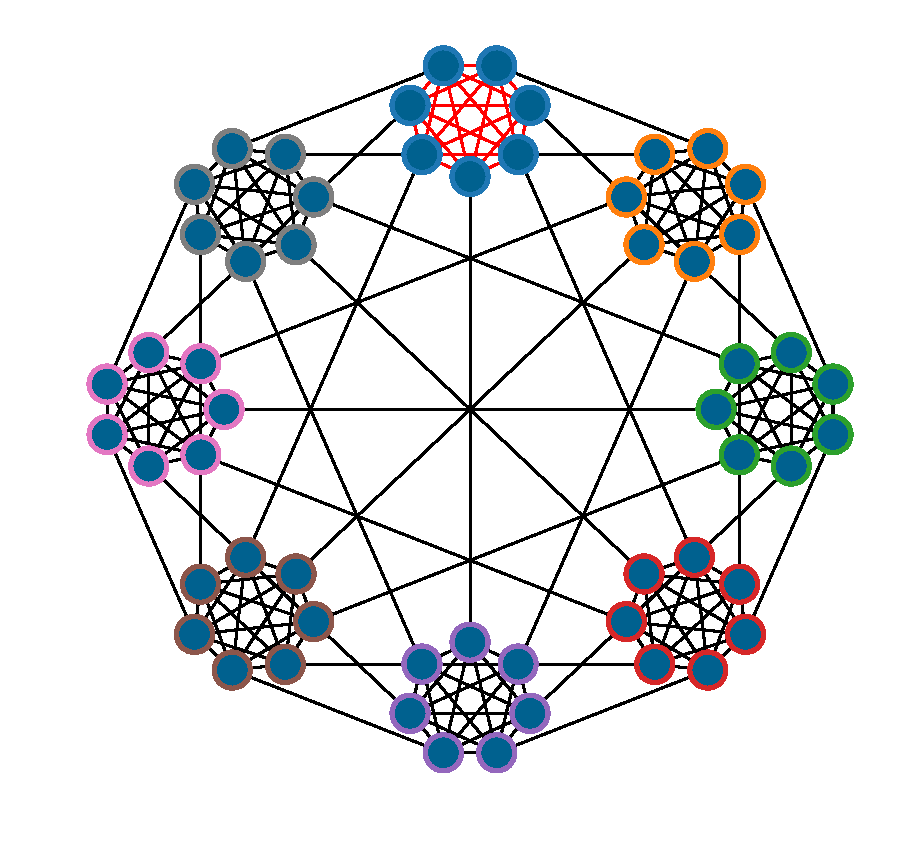
\includegraphics[width=.8\linewidth]{network2.pdf}
								\caption{An example of our network architecture.}
								\label{fig:network}
							\end{figure}
						\end{block}		
										
						\vfill
						\begin{block}{Neuronal dynamics}
							We use a rate-encoding model, in which each neuron has a membrane potential $x_j$, a sigmoidal activation function $\sigma$ and receives excitatory input $E_j$ and inhibitory $I_j$:
							\begin{gather*}
								\tau_x \dot{x}_j = -x_j + E_j + I_j\\
								y_j = \sigma \left(x_k\right) = \frac{1}{1+\exp \left(-a x_k \right) } \\
								E_j = \sum_{k} w_{jk} y_k \\
								I_j = \sum_k z_{jk} \tilde{y}_k \\
								\label{eq:neuron}
							\end{gather*}
							\begin{figure}
								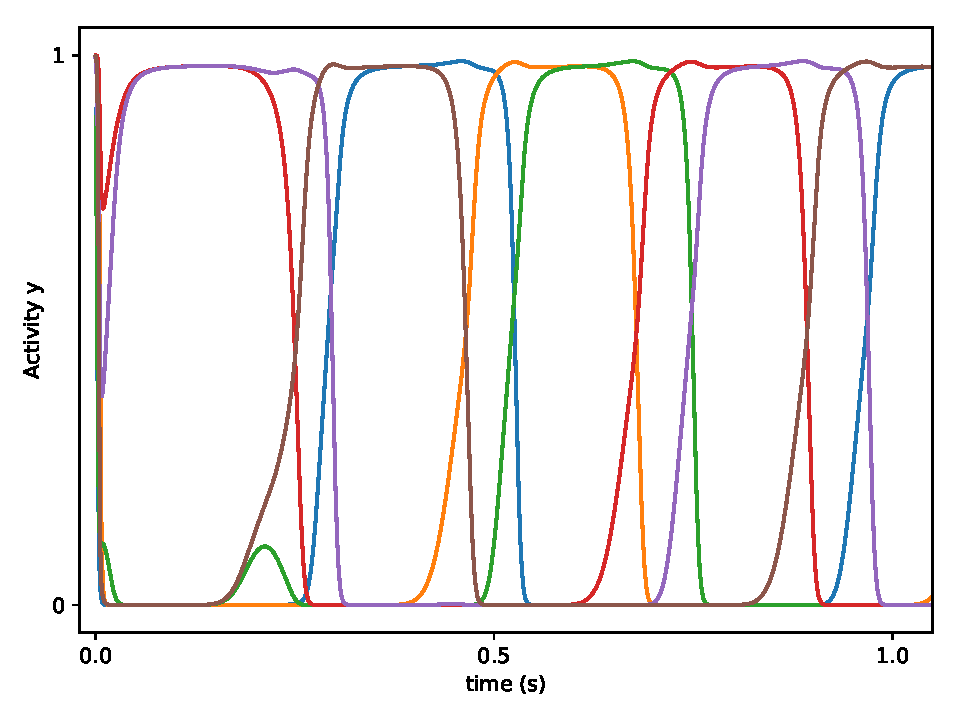
\includegraphics[width=.8\linewidth]{ring_activity2}
								\caption{Example activity on a ring of 6 neurons, with nearest neighbour excitatory connections.}
							\end{figure}
							
						\end{block}
						
						
						
						\vfill
						\begin{emphblock}{Conclusions}
							\singleitem{That is really important to keep in mind.}
							\singleitem{Furthermore ...}
						\end{emphblock}
						%\vfill
						%%% END CONTENT of column 1 %%%

					 } % end of parbox
				\end{minipage}
			%\end{beamercolorbox}
		\end{column}
		% ---------------------------------------------------------%
		% end of column 1
		%\hfil
		% ---------------------------------------------------------%
		% Set up a column 2
		\begin{column}{.64\textwidth}
			%\begin{beamercolorbox}[center,wd=\textwidth]{postercolumn}
				\begin{minipage}[T]{.95\textwidth}
					\parbox[t][\columnheight]{\textwidth}{

					%%% CONTENT of column 2 %%%
					%\vfill
					\begin{block}{Full depletion model}
						\begin{columns}
							\begin{column}[T]{.5\textwidth}
							\begin{figure}
								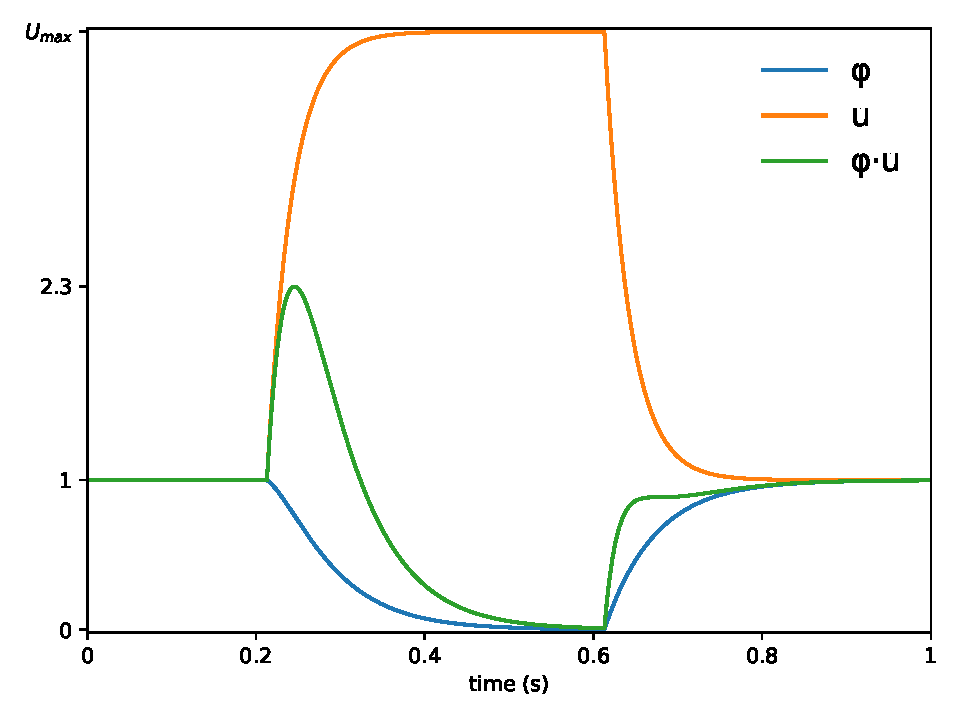
\includegraphics[width=1\linewidth]{full_depletion.pdf}
								\caption{Dynamics of the full depletion model, with high presynaptic activity.}
								\label{fig:full_depletion}
							\end{figure}	
							\end{column}							
							
							\begin{column}[T]{.5\textwidth}
								To enforce the transient state dynamics, the winning clique state has to become unstable after some time. 
								
								This is achieved by lowering inhibitory signals in case of sustained activity, through the \emph{full depletion model}, that is inspired by the Tsodyks-Markram model \cite{tsodyks2008model}.
								
								The pre-synaptic activity $\tilde{y}_j$ is proportional to the somatic activity $y_j$, through two terms $u_j$ and $\varphi_j$.
								
								$u_j$ represents the likelihood of neurotransmitter release, which increases with high inputs, while $\varphi_j$ represents the concentration of available vesicles, that decreases while firing, according to the following dynamics:						
								\begin{gather*}
									\tilde{y}_j = y_j u_j \varphi_j \\
									\dot{u}_j = \frac{U_y -u}{T_u}, \quad U_y = 1 + \left( U_\text{max} -1 \right) y_j\\ 
									\dot{\varphi}_j = \frac{\varPhi_u - \varphi}{T_\varphi}, \quad \varPhi_u = 1- \frac{u y_j}{U_\text{max}} \\	
								\end{gather*}

							\end{column}
						\end{columns}
					\end{block}
					
					\begin{block}{Sensory input}
						\begin{columns}
							\begin{column}[T]{.1\textwidth}
									\begin{figure}[T]
										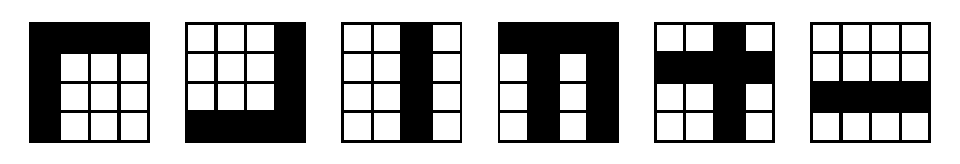
\includegraphics[width=3.5\textwidth, angle=-90]{input_ex6.pdf}
																		
									\end{figure}
							\end{column}
							
							\begin{column}[T]{.9\textwidth}
								We want our network to extract information from an external environment via signal separation and feature extraction. An example would be to identify recurring patterns and to separate them, even if they occur simultaneously.
													
								We use the bars problem, in which horizontal and vertical bars are presented on a retina of L x L pixels. Bars are independently drawn so that there is, on average, one bar per input. Active bar pixels have $y_l^{\text{ext}}=1$, and inactive ones $y_l^{\text{ext}}=0$, as shown in the Figure.
														
								The bar intersection pixels also have value 1, so that a non linear independent component analysis has to be performed in order to separate bars.
								
								This sensory input layer is connected to the network with excitatory connections $v_{jl}$ so that an extra input term $\Delta E_j$ is added:
								\begin{equation*}
									\Delta E_j = \sum_{l=1}^{L^2} v_{jl} y_l^{\text{ext}}
								\end{equation*}
								The initial weights are chosen so that, on average, $\Delta E_j \approx 0.5$. With these weights external input can, on average, change the internal dynamics only when the short-term plasticity tunes down inhibitory weights.
							
							\end{column}
						\end{columns}

							

					\end{block}
						
					\begin{block}{Learning rule}
						\begin{columns}
							\begin{column}[T]{.5\textwidth}
								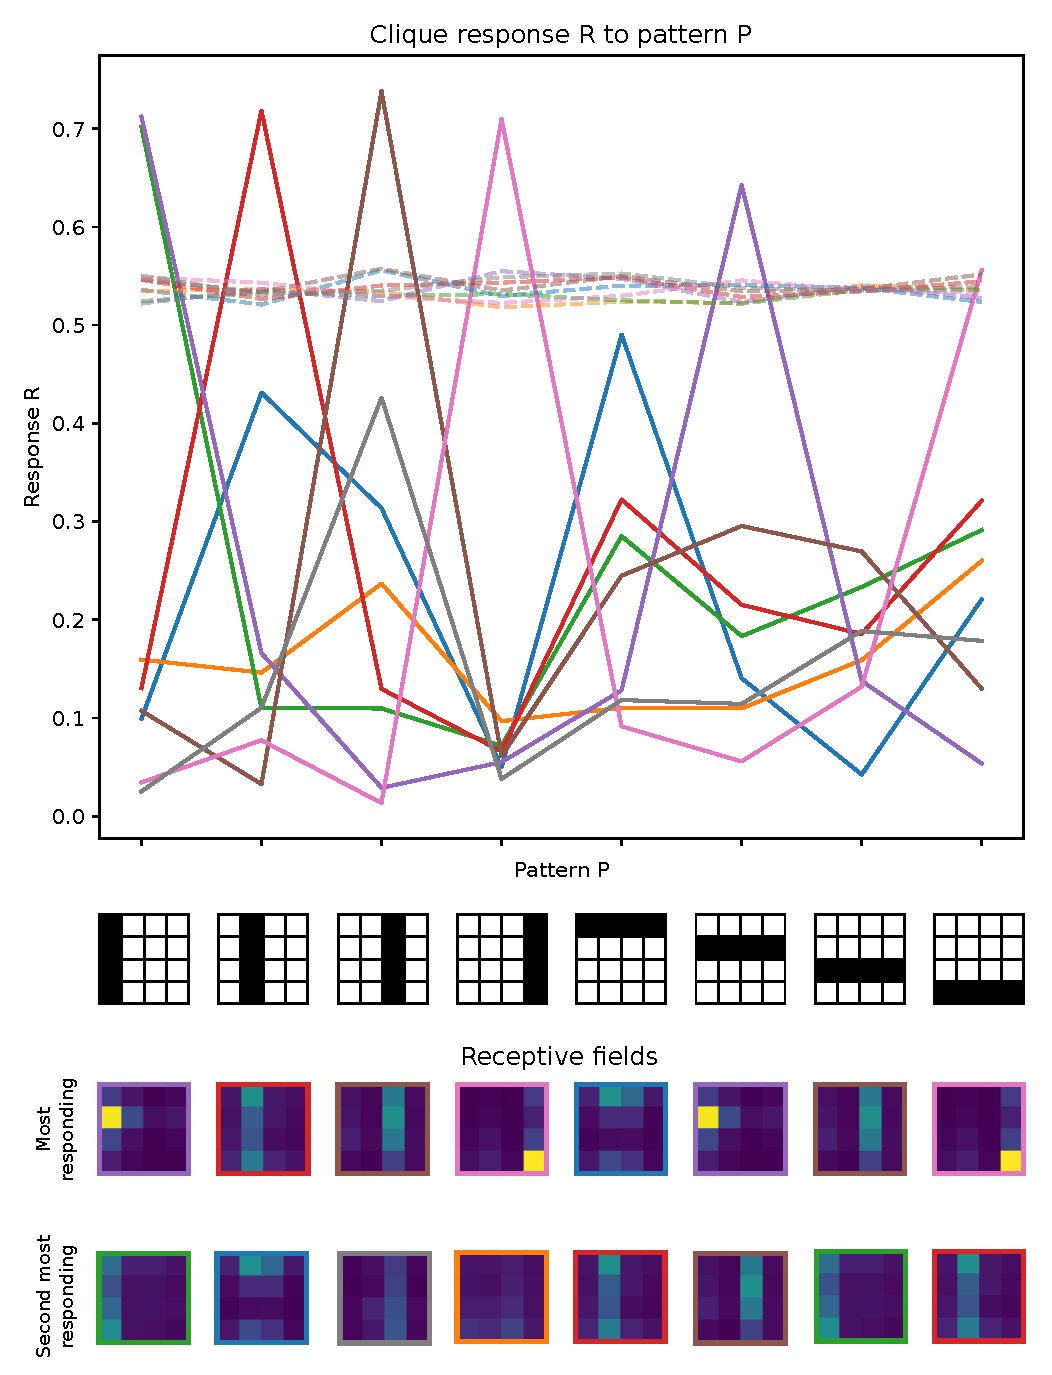
\includegraphics[width=1\linewidth]{complete2.pdf}	
							\end{column}								
							
							\begin{column}[T]{.5\textwidth}
								
							\end{column}
						\end{columns}
							
										
					\end{block}
						

					\vfill
					\begin{refblock}{References}
						\begin{columns}
						 \begin{thebibliography}{1}
								\begin{column}[T]{.46\textwidth}
									\bibitem{fiser2004modulation}
										Fiser et al., Small modulation of ongoing cortical dynamics by sensory input during natural vision.
										\emph{Nature}, 2004.
										
									\bibitem{gros2017semantic}
									Gros and Kaczor, Semantic learning in autonomously active recurrent neural network.
									\emph{Logic Journal of the IGPL}, 2017.										
								\end{column}
								\begin{column}[T]{.46\textwidth}
									\bibitem{tsodyks2008model}
									Mongillo et al., Synaptic theory of working memory.
									\emph{Science}, 2008
								\end{column}
						 \end{thebibliography}
						\end{columns}
					\end{refblock}
					%\vfil
					%%% END CONTENT of column 2 %%%


					} % end of parbox
					% ---------------------------------------------------------%
					% end the column
				\end{minipage}
			%\end{beamercolorbox}
		\end{column}
		% ---------------------------------------------------------%
		% end of column 2
	\end{columns}
	\hfill
	\vskip1ex
\end{frame}
\end{document}
